\ifx\allfiles\undefined
\documentclass[12pt, a4paper,oneside, UTF8]{ctexbook}
\usepackage[dvipsnames]{xcolor}
\usepackage{amsmath}   % 数学公式
\usepackage{amsthm}    % 定理环境
\usepackage{amssymb}   % 更多公式符号
\usepackage{graphicx}  % 插图
%\usepackage{mathrsfs}  % 数学字体
%\usepackage{newtxtext,newtxmath}
%\usepackage{arev}
\usepackage{kmath,kerkis}
\usepackage{newtxtext}
\usepackage{bbm}
\usepackage{enumitem}  % 列表
\usepackage{geometry}  % 页面调整
%\usepackage{unicode-math}
\usepackage[colorlinks,linkcolor=black]{hyperref}


\usepackage{ulem}	   % 用于更多的下划线格式,
					   % \uline{}下划线,\uuline{}双下划线,\uwave{}下划波浪线,\sout{}中间删除线,\xout{}斜删除线
					   % \dashuline{}下划虚线,\dotuline{}文字底部加点


\graphicspath{ {flg/},{../flg/}, {config/}, {../config/} }  % 配置图形文件检索目录
\linespread{1.5} % 行高

% 页码设置
\geometry{top=25.4mm,bottom=25.4mm,left=20mm,right=20mm,headheight=2.17cm,headsep=4mm,footskip=12mm}

% 设置列表环境的上下间距
\setenumerate[1]{itemsep=5pt,partopsep=0pt,parsep=\parskip,topsep=5pt}
\setitemize[1]{itemsep=5pt,partopsep=0pt,parsep=\parskip,topsep=5pt}
\setdescription{itemsep=5pt,partopsep=0pt,parsep=\parskip,topsep=5pt}

% 定理环境
% ########## 定理环境 start ####################################
\theoremstyle{definition}
\newtheorem{defn}{\indent 定义}[section]

\newtheorem{lemma}{\indent 引理}[section]    % 引理 定理 推论 准则 共用一个编号计数
\newtheorem{thm}[lemma]{\indent 定理}
\newtheorem{corollary}[lemma]{\indent 推论}
\newtheorem{criterion}[lemma]{\indent 准则}

\newtheorem{proposition}{\indent 命题}[section]
\newtheorem{example}{\indent \color{SeaGreen}{例}}[section] % 绿色文字的 例 ,不需要就去除\color{SeaGreen}{}
\newtheorem*{rmk}{\indent \color{red}{注}}

% 两种方式定义中文的 证明 和 解 的环境:
% 缺点:\qedhere 命令将会失效【技术有限,暂时无法解决】
\renewenvironment{proof}{\par\textbf{证明.}\;}{\qed\par}
\newenvironment{solution}{\par{\textbf{解.}}\;}{\qed\par}

% 缺点:\bf 是过时命令,可以用 textb f等替代,但编译会有关于字体的警告,不过不影响使用【技术有限,暂时无法解决】
%\renewcommand{\proofname}{\indent\bf 证明}
%\newenvironment{solution}{\begin{proof}[\indent\bf 解]}{\end{proof}}
% ######### 定理环境 end  #####################################

% ↓↓↓↓↓↓↓↓↓↓↓↓↓↓↓↓↓ 以下是自定义的命令  ↓↓↓↓↓↓↓↓↓↓↓↓↓↓↓↓

% 用于调整表格的高度  使用 \hline\xrowht{25pt}
\newcommand{\xrowht}[2][0]{\addstackgap[.5\dimexpr#2\relax]{\vphantom{#1}}}

% 表格环境内长内容换行
\newcommand{\tabincell}[2]{\begin{tabular}{@{}#1@{}}#2\end{tabular}}

% 使用\linespread{1.5} 之后 cases 环境的行高也会改变,重新定义一个 ca 环境可以自动控制 cases 环境行高
\newenvironment{ca}[1][1]{\linespread{#1} \selectfont \begin{cases}}{\end{cases}}
% 和上面一样
\newenvironment{vx}[1][1]{\linespread{#1} \selectfont \begin{vmatrix}}{\end{vmatrix}}

\def\d{\textup{d}} % 直立体 d 用于微分符号 dx
\def\R{\mathbb{R}} % 实数域
\def\N{\mathbb{N}} % 自然数域
\def\C{\mathbb{C}} % 复数域
\def\Z{\mathbb{Z}} % 整数环
\def\Q{\mathbb{Q}} % 有理数域
\newcommand{\bs}[1]{\boldsymbol{#1}}    % 加粗,常用于向量
\newcommand{\ora}[1]{\overrightarrow{#1}} % 向量

% 数学 平行 符号
\newcommand{\pll}{\kern 0.56em/\kern -0.8em /\kern 0.56em}

% 用于空行\myspace{1} 表示空一行 填 2 表示空两行  
\newcommand{\myspace}[1]{\par\vspace{#1\baselineskip}}

%s.t. 用\st就能打出s.t.
\DeclareMathOperator{\st}{s.t.}

%罗马数字 \rmnum{}是小写罗马数字, \Rmnum{}是大写罗马数字
\makeatletter
\newcommand{\rmnum}[1]{\romannumeral #1}
\newcommand{\Rmnum}[1]{\expandafter@slowromancap\romannumeral #1@}
\makeatother
\begin{document}
	% \title{{\Huge{\textbf{$Complex \,\, Analysis$\footnote{课堂教材:\textbf{《$Complex \,\, Analysis$》---  $Elias \,\, M. \,\, Stein$}}}}}}
\author{$-TW-$}
\date{\today}
\maketitle                   % 在单独的标题页上生成一个标题

\thispagestyle{empty}        % 前言页面不使用页码
\begin{center}
	\Huge\textbf{序}
\end{center}


\vspace*{3em}
\begin{center}
	\large{\textbf{天道几何,万品流形先自守;}}\\
	
	\large{\textbf{变分无限,孤心测度有同伦。}}
\end{center}

\vspace*{3em}
\begin{flushright}
	\begin{tabular}{c}
		\today \\ \small{\textbf{长夜伴浪破晓梦,梦晓破浪伴夜长}}
	\end{tabular}
\end{flushright}


\newpage                      % 新的一页
\pagestyle{plain}             % 设置页眉和页脚的排版方式(plain:页眉是空的,页脚只包含一个居中的页码)
\setcounter{page}{1}          % 重新定义页码从第一页开始
\pagenumbering{Roman}         % 使用大写的罗马数字作为页码
\tableofcontents              % 生成目录

\newpage                      % 以下是正文
\pagestyle{plain}
\setcounter{page}{1}          % 使用阿拉伯数字作为页码
\pagenumbering{arabic}
\setcounter{chapter}{-1}    % 设置 -1 可作为第零章绪论从第零章开始 
	\else
	\fi
	%  ############################ 正文部分

\chapter{$Week \,\, 5$}
\section{闭路变形原理}
\paragraph{围道}
为了叙述方便,我们将简单闭曲线记作\textbf{围道(contour)}. 并默认其为正向.
\begin{defn}\label{def 5.1.1}
	A simple closed path is called a \underline{\textcolor{blue}{\textbf{contour}}}. If nothing is specified, we'll assume the contour is positively oriented.
\end{defn}

\vspace{2em}
\paragraph{闭路变形原理}
下面来介绍\textbf{闭路变形原理}.(实际上可视为Cauchy's Theorem 的推论)
\begin{thm}\label{thm 5.1.1}
	\textbf{Principle of contour deformation}.\\
	Let $\Omega \subset \C$ be open, $f : \Omega \longrightarrow \C$ be holomorphic. Let $\gamma_1$ be a contour in $\Omega$, $\gamma_2$ be another contour in $\Omega \cap Interior(\gamma_1)$. If $Interior(\gamma_1) \cap Exterior(\gamma_2) \subset \Omega$, then
	\begin{align}
		\int_{\gamma_1}{f(z) dz} = \int_{\gamma_2}{f(z) dz}
	\end{align}
	
	\vspace{1em}
	\begin{rmk}
		条件$Interior(\gamma_1) \cap Exterior(\gamma_2) \subset \Omega$ 保证了$\gamma_1$ 与$\gamma_2$ 之间围成的区域不存在空洞(亏格),从而在这片区域上Cauchy's Theorem 总是奏效的.
	\end{rmk}
	
	\begin{figure}[htbp]  %h此处,t页顶,b页底,p独立一页,浮动体出现的位置
		\centering  %图表居中
		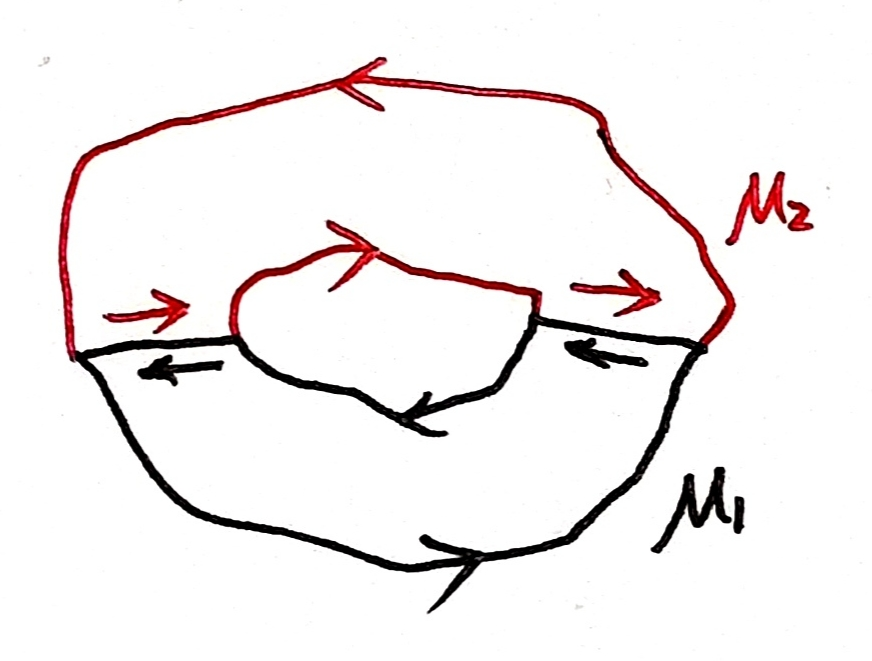
\includegraphics[width=0.3\textwidth]{figure/5.1-1} %图片的名称或者路径之中有空格会出问题 
		\caption{\textbf{Principle of contour deformation}} % 图片标题
		\label{pic 5.1-1}
	\end{figure}
	
	\vspace{2em}
	\begin{proof}
		\begin{align}
			\int_{\gamma_1}{f(z) dz} - \int_{\gamma_2}{f(z) dz} 
			&= \int_{\gamma_1}{f(z) dz} + \int_{\gamma_{2}^{-}}{f(z) dz} \\
			&= \int_{\mu_1}{f(z) dz} + \int_{\mu_2}{f(z) dz} = 0 + 0 = 0
		\end{align}
	\end{proof}	
\end{thm}

\vspace{2em}
下面给出Thm \ref{thm 5.1.1} 的一种Special Case. (Interior($\gamma_1$)仅有一点不在$\Omega$ 内)
\begin{corollary}\label{cor 5.1.2}
	Let $\Omega \subset \C$ be open, $f : \Omega \longrightarrow \C$ be holomorphic. Let $\gamma$ be a contour in $\Omega$ and $\exists \alpha \in Interior(\gamma)$, $\st Interior(\gamma) \backslash \{ \alpha \} \subset \C$. Then
	\begin{align}
		\int_{\gamma}{f(z) dz} = \int_{C_{r}(\alpha)}{f(z) dz} , \,\, where \,\, C_{r}(\alpha) \subset Interior(\gamma)
	\end{align}
\end{corollary}

\vspace{2em}
下面给出更一般的表述.(Interior($\gamma$)内有有限个点不在$\Omega$ 内)
\begin{corollary}\label{cor 5.1.3}
	Let $\Omega \subset \C$ be open, $f : \Omega \longrightarrow \C$ be holomorphic and $\gamma$ is a contour in $\Omega$. If $\alpha_1 , \cdots , \alpha_n \in Interior(\gamma)$, such $Interior(\gamma) \backslash \{ \alpha_1 , \cdots , \alpha_n \} \subset \Omega$, then
	\begin{align}
		\int_{\gamma}{f(z) dz} = \sum_{k = 1}^{n}{\int_{C_{r_k}(\alpha_k)}{f(z) dz}} 
	\end{align}
	where $C_{r_k}(\alpha_k)$ are disjoint “small” circles.
	
	\begin{figure}[htbp]  %h此处,t页顶,b页底,p独立一页,浮动体出现的位置
		\centering  %图表居中
		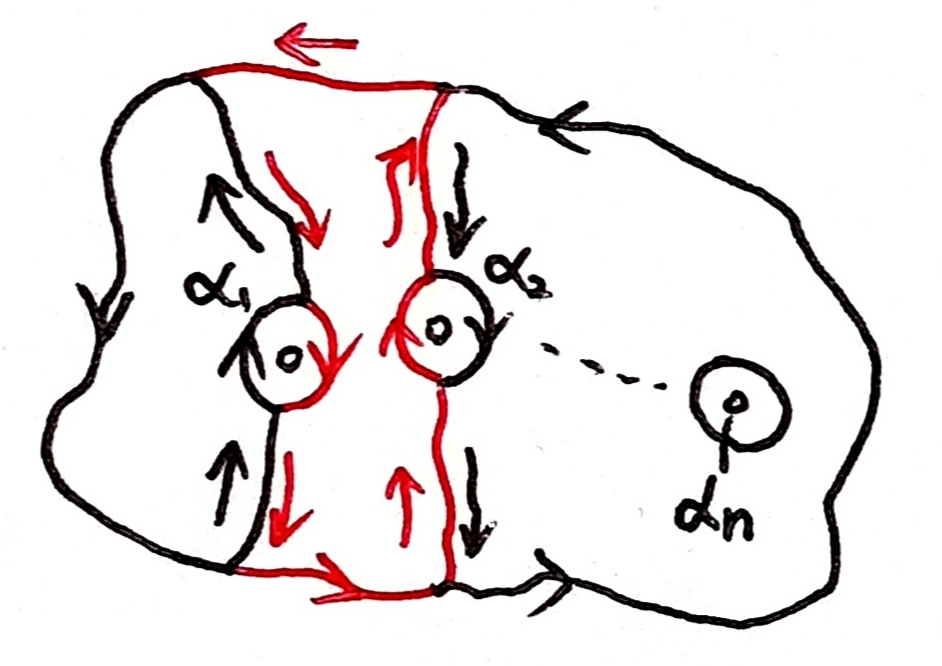
\includegraphics[width=0.3\textwidth]{figure/5.1-2} %图片的名称或者路径之中有空格会出问题 
		\caption{\textbf{Principle of contour deformation (Special Case)}} % 图片标题
		\label{pic 5.1-2}
	\end{figure}
	
	\begin{proof}
		即证
		\begin{align}
			\int_{\gamma}{f(z) dz} + \sum_{k = 1}^{n}{\int_{C_{r_k}^{-}(\alpha_k)}{f(z) dz}} = \sum_{k = 1}^{n}{\int_{\mu_{k}}{f(z) dz}} = \sum_{k = 1}^{n}{0} = 0
		\end{align}
	\end{proof}
\end{corollary}

\newpage
\section{$Cauchy \,\, Integral \,\, Formulas$}
\begin{center}
	接下来我们介绍另一个计算环路积分非常重要的公式——\textbf{Cauchy Integral Formulas}.
\end{center}

\paragraph{Cauchy Integral Formulas}
首先给出一个命题.
\begin{proposition}\label{prop 5.2.1}
	Let $\Omega \subset \C$ be open, $f : \Omega \longrightarrow \C$ be holomorphic, $\gamma$ be a contour in $\Omega$. Assume $\exists \alpha \in Interior(\gamma)$, $\st$
	\begin{align}
		Interior(\gamma) \backslash \{ \alpha \} \subset \Omega \,\,\,\, and \,\,\,\, \lim_{z \to \alpha}{(z - \alpha)f(z)} = 0
	\end{align}
	Then
	\begin{align}
		\int_{\gamma}{f(z) dz} = 0
	\end{align}
	
	\vspace{2em}
	\begin{proof}
		$\forall \epsilon > 0$, $\exists \delta > 0$, $\st$
		\begin{align}
			\left| z - \alpha \right| < \delta \,\, \Rightarrow \,\, \left| (z - \alpha) f(z) \right| < \epsilon
		\end{align}
		By the \textbf{principle of contour deformation} (Thm \ref{thm 5.1.1}),
		\begin{align}
			\int_{\gamma}{f(z) dz} = \int_{C_{r}(\alpha)}{f(z) dz} , \,\, where \,\, 0 < r < \delta
		\end{align}
		Then
		\begin{align}
			\left| \int_{\gamma}{f(z) dz} \right| 
			\leq \sup_{z \in C_{r}(\alpha)}{\left| f(z) \right|} \cdot length(\gamma) 
			&= \sup_{z \in C_{r}(\alpha)}{\left| f(z) \right|} \cdot 2 \pi r \\
			&< \frac{\epsilon}{r} \cdot 2 \pi r = 2 \pi \epsilon
		\end{align}
	\end{proof}
\end{proposition}

\newpage
下面给出\textbf{Cauchy Integral Formulas}.
\begin{thm}\label{thm 5.2.1}
	\textbf{CIF}.\\
	Let $\Omega \subset \C$ be open, $f : \Omega \longrightarrow \C$ be holomorphic. Then for any $z_0 \in \Omega$,
	\begin{align}
		f(z_0) = \frac{1}{2 \pi i} \int_{\gamma}{\frac{f(\zeta)}{\zeta - z_0} d\zeta}
	\end{align}
	where $\gamma$ is any contour in $\Omega$ $\st$ $z_0 \in Interior(\gamma) \subset \Omega$.
	
	\vspace{2em}
	\begin{proof}
		Let
		\begin{align}
			g(z) = \frac{f(z) - f(z_0)}{z - z_0}
		\end{align}
		Then $g(z)$ is holomorphic on $\Omega \backslash \{ z_0 \}$. Clearly
		\begin{align}
			\lim_{z \to z_0}{(z - z_0) g(z)} = 0 , \,\, Interior(\gamma) \backslash \{ z_0 \} \subset \Omega \backslash \{ z_0 \}
		\end{align}
		By Prop \ref{prop 5.2.1},
		\begin{align}
			\int_{\gamma}{g(z) dz} = 0 \,\, \Rightarrow \,\, \int_{\gamma}{\frac{f(z)}{z - z_0} dz} = \int_{\gamma}{\frac{f(z_0)}{z - z_0} dz}
		\end{align}
		Therefore
		\begin{align}
			\int_{\gamma}{\frac{f(z)}{z - z_0} dz} 
			= \int_{\gamma}{\frac{f(z_0)}{z - z_0} dz} 
			= f(z_0) \int_{\gamma}{\frac{1}{z - z_0} dz} 
			&= f(z_0) \int_{C_{r}(z_0)}{\frac{1}{z - z_0} dz} \\
			&= 2 \pi i \cdot f(z_0)
		\end{align}
	\end{proof}
\end{thm}

\vspace{2em}
Therefore, according to Cauchy Integral Formulas, we get
\begin{align}
	f(z) = \frac{1}{2 \pi i} \int_{\gamma}{\frac{f(\zeta)}{\zeta - z} d\zeta} 
\end{align}
\begin{center}
	where $f$ is holomorphic on an open set containing the contour $\gamma$ and its interior, $z \in Interior(\gamma)$.
\end{center}

\newpage
\paragraph{高阶Cauchy Integral Formulas}
下面给出\textbf{高阶}的Cauchy Integral Formulas.
\begin{thm}\label{thm 5.2.2}
	Let $\Omega \subset \C$ be open, $f : \Omega \longrightarrow \C$ be holomorphic. Then $f$ is complex differentiable to all orders and moreover, $\forall z \in \Omega$
	\begin{align}
		f^{(n)}(z) = \frac{n!}{2 \pi i} \int_{\gamma}{\frac{f(\zeta)}{(\zeta - z)^{n + 1}} d\zeta} , \,\, n = 0 , 1 , 2 , \cdots
	\end{align}
	where $\gamma$ is any contour in $\Omega$ $\st$ $z \in Interior(\gamma) \subset \Omega$.
\end{thm}

\vspace{2em}
\paragraph{\textbf{Cauchy's Inequalities}}
作为\textbf{柯西积分公式 (CIF)}的推论,下面可得到\textbf{Cauchy's Inequalities}.
\begin{corollary}\label{cor 5.2.3}
	\textbf{Cauchy's Inequalities}.\\
	If $f$ is holomorphic on an open set $\Omega$ with $D_{R}(z_0) \subset \Omega$, $R > 0$, then
	\begin{align}
		\left| f^{(n)}(z_0) \right| \leq \frac{n! \,\, \Vert f \Vert_{C_{R}(z_0)}}{R^n} , \,\, where \,\, \Vert f \Vert_{C_{R}(z_0)} = \sup_{z \in C_{R}(z_0)}{\left| f(z) \right|}
	\end{align}
\end{corollary}

\vspace{2em}
\paragraph{\textbf{Liouville's therom}}
下面给出\textbf{CIF} 的另一条重要推论. 在此之前,先给出\textbf{整函数 (entire)}的定义.
\begin{defn}\label{def 5.2.1}
	A holomorphic function defined on the whole $\C$ is called an \underline{\textcolor{blue}{\textbf{entire function}}}.
\end{defn}

\vspace{2em}
下面给出\textbf{刘维尔定理 (Liouville's theorem)}的内容.
\begin{corollary}\label{cor 5.2.4}
	\textbf{Liouville's theorem}.
	\begin{center}
		If $f$ is entire and bounded, then $f$ is constant.
	\end{center}
	
	\vspace{2em}
	\begin{proof}
		$\forall z \in \C$, by \textbf{Cauchy's Inequalities (Cor \ref{cor 5.2.3})}
		\begin{align}
			\left| f^{'}(z) \right| \leq \frac{\Vert f \Vert_{\C}}{R} \leq \frac{M}{R} , \,\, where \,\, \left| f \right| \leq M
		\end{align}
		Letting $R \to \infty$, we get $f^{'}(z) = 0$, $\forall z \in \C$ $\,\, \Rightarrow \,\,$ $f$ is constant.
	\end{proof}
\end{corollary}

\newpage
\paragraph{具有原函数的充要条件}
下面在定理 \ref{thm 4.1.3} 的基础上,再增加一条具有原函数的充要条件.
\begin{thm}\label{thm 5.2.5}
	Let $\Omega \subset \C$ be a region, $f : \Omega \longrightarrow \C$ be continuous. Then \textbf{TFAE} \\
	(the followings are equivalent):
	\begin{enumerate}
		\item[(1)]$f$ admits a primitive on $\Omega$.
		
		\item[(2)]$\forall \alpha , \beta \in \Omega$, $\int_{\gamma}{f(z) dz}$ is invariant for any path.
		
		\item[(3)]$\forall \alpha , \beta \in \Omega$, $\int_{\gamma}{f(z) dz}$ is invariant for any zig-zag path.
		
		\item[(4)]$\int_{\gamma}{f(z) dz} = 0$ for any closed path $\gamma \subset \Omega$. 
	\end{enumerate}
	
	\vspace{2em}
	\begin{proof}
		$(4) \Rightarrow (2)$: Fix $\alpha , \beta \in \Omega$, $\forall$ two paths $\gamma_1 , \gamma_2 \subset \Omega$ joining $\alpha$ to $\beta$, by (4)
		\begin{align}
			\int_{\gamma_1}{f(z) dz} - \int_{\gamma_2}{f(z) dz} = \int_{\gamma_1 \circ \gamma_{2}^{-}}{f(z) dz} = 0 , \,\, where \,\, \gamma_1 \circ \gamma_{2}^{-} \,\, is \,\, a  \,\, closed \,\, path \,\, in \,\, \Omega
		\end{align}
		Therefore
		\begin{align}
			\int_{\gamma_1}{f(z) dz} = \int_{\gamma_2}{f(z) dz} , \,\, \forall \gamma_1 , \gamma_2 \subset \Omega
		\end{align}
	\end{proof}
\end{thm}

\vspace{2em}
\paragraph{\textbf{Morera's Theorem}}
有了具有原函数的充要条件之后 (Thm \ref{thm 5.2.5}),下面我们可以对全纯函数进行充要刻画,此即为\textbf{Morera's Theorem} 的推广.

\begin{proposition}\label{prop 5.2.2}
	Let $\Omega \subset \C$ be \textbf{simply connected}, $f : \Omega \longrightarrow \C$ be continuous. Then \textbf{TFAE}
	\begin{enumerate}
		\item[(1)]$f$ is holomorphic on $\Omega$.
		
		\item[(2)]$\int_{\gamma}{f(z) dz} = 0$ for any closed path $\gamma \subset \Omega$. 
	\end{enumerate}
	
	\vspace{1em}
	\begin{rmk}
		命题中$(2) \Rightarrow (1)$ 的部分即为\textbf{Morera's Theorem}.
	\end{rmk}
	
	\vspace{1em}
	\begin{proof}
		$(1) \Rightarrow (2)$: is by \textbf{Cauchy's Theorem} (Thm \ref{thm 4.3.2}). \\
		$(2) \Rightarrow (1)$: By Thm \ref{thm 5.2.5}, $f$ admits a primitive $F$ on $\Omega$, i.e. $F^{'} = f$, then $F$ is holomorphic on $\Omega$. \\
		By \textbf{CIF} (Thm \ref{thm 5.2.2}), $F$ is infinitely complex differentiable. \\
		In particular, $F$ is twice complex differentiable. $\Rightarrow$ $F^{''} = f^{'}$ $\Rightarrow$ $f$ is holomorphic on $\Omega$. 
	\end{proof}
\end{proposition}

\newpage
由\textbf{命题 \ref{prop 5.2.2}}可直接得到如下推论.
\begin{corollary}\label{cor 5.2.6}
	Every holomorphic function on a simply connected region admits a primitive.
\end{corollary}

\vspace{2em}
在利用\textbf{命题 \ref{prop 5.2.2} (Morera's Thereom)}判定函数全纯时,要注意条件 (2)中道路$\gamma$ 的\textbf{任意性}. 下面便给出一个反例.
\begin{example}\label{ex 5.2.1}
	Suppose $\int_{C_{r}(0)}{f(z) dz} = 0$ for all $0 < r < 1$, can we conclude $f$ is holomorphic on $\mathbb{D}$?
	
	\vspace{2em}
	\begin{solution}
		The answer is absolutely No. Take $f(z) = \left| z \right|^2$. Then $\int_{C_{r}(0)}{f(z) dz} = 0$, $\forall 0 < r < 1$. \\
		Since
		\begin{align}
			f(z) = \left| z \right|^2 = z \cdot \overline{z} , \,\, \frac{\partial f}{\partial \overline{z}} = z \neq 0 , \,\, \forall z \in \C \backslash \{ 0 \}
		\end{align}
		Therefore, $f$ is not holomorphic on $\mathbb{D}$.
		
		\begin{rmk}
			事实上,取道路$\gamma$ 为以原点为圆心,$\frac{1}{2}$ 为半径的上半圆,逆时针方向,可证$\int_{\gamma}{f(z) dz} \neq 0$.
		\end{rmk}
	\end{solution}
\end{example}






\newpage
\section{课堂例题$2024-03-25$}
\begin{enumerate}
	\item Evaluate 
	\begin{align}
		\int_{\gamma}{\frac{2z - 1}{z^2 - z} dz}
	\end{align}
	where $\gamma$ is any contour $\st$ $\overline{\mathcal{D}} \subset Interior(\gamma)$.
	
	\vspace{2em}
	\begin{solution}
		By Cor \ref{cor 5.1.3},(\textbf{闭路变形原理})
		\begin{align}
			\int_{\gamma}{f(z) dz} 
			&= \int_{C_{\frac{1}{3}}(0)}{f(z) dz} + \int_{C_{\frac{1}{3}}(1)}{f(z) dz} \\
			&= \int_{C_{\frac{1}{3}}(0)}{(\frac{1}{z - 1} + \frac{1}{z}) dz} + \int_{C_{\frac{1}{3}}(1)}{(\frac{1}{z - 1} + \frac{1}{z}) dz}
		\end{align}
		Since $\frac{1}{z - 1}$ is holomorphic on \textcolor{red}{$Interior(C_{\frac{1}{3}}(0)) = D_{\frac{1}{3}}(0)$}, where $D_{\frac{1}{3}}(0)$ is simply connected, then \\
		by Cauchy's Theorem,
		\begin{align}
			\int_{C_{\frac{1}{3}}(0)}{(\frac{1}{z - 1} + \frac{1}{z}) dz} = \int_{C_{\frac{1}{3}}(0)}{\frac{1}{z} dz}
		\end{align}
		Similarly, since $\frac{1}{z}$ is holomorphic on $D_{\frac{1}{3}}(1)$, then
		\begin{align}
			\int_{C_{\frac{1}{3}}(1)}{(\frac{1}{z - 1} + \frac{1}{z}) dz} = \int_{C_{\frac{1}{3}}(1)}{\frac{1}{z - 1} dz}
		\end{align}
		Therefore
		\begin{align}
			\int_{\gamma}{f(z) dz} 
			&= \int_{C_{\frac{1}{3}}(0)}{(\frac{1}{z - 1} + \frac{1}{z}) dz} + \int_{C_{\frac{1}{3}}(1)}{(\frac{1}{z - 1} + \frac{1}{z}) dz} \\
			&= \int_{C_{\frac{1}{3}}(0)}{\frac{1}{z} dz} + \int_{C_{\frac{1}{3}}(1)}{\frac{1}{z - 1} dz} \\
			&= 2\pi i + 2\pi i \\
			&= 4 \pi i
		\end{align}
	\end{solution}
	
	\newpage
	
	\item Evaluate
	\begin{align}
		&\int_{C_{3}(0)}{\frac{e^{z^2}}{z - 2} dz} \,\,\,\, ( = 2 \pi i f(z_0) = 2 \pi i e^4) \\
		&\int_{C_{1}(0)}{\frac{e^{z^2}}{z - 2} dz} \,\,\,\, ( = 0)
	\end{align}
	
	\vspace{2em}
	
	\item Evaluate
	\begin{align}
		\int_{C_{2}(0)}{\frac{\sin{z}}{z^2 + 1} dz}
	\end{align}
	
	\vspace{2em}
	\begin{solution}
		\begin{align}
			\int_{C_{2}(0)}{\frac{\sin{z}}{z^2 + 1} dz} 
			&= \int_{C_{\frac{1}{2}}(i)}{\frac{\sin{z}}{z + i} \cdot \frac{1}{z - i} dz} + \int_{C_{\frac{1}{2}}(-i)}{\frac{\sin{z}}{z - i} \cdot \frac{1}{z + i} dz} \\
			&= 2 \pi i \cdot \frac{\sin{i}}{2i} + 2 \pi i \cdot \frac{\sin{(-i)}}{-2i} \\
			&= 2\pi \sin{i}
		\end{align}
	\end{solution}
	
	\vspace{2em}
	
	\item Evaluate
	\begin{align}
		\int_{C_{3}(0)}{\frac{z}{(z - 1)(z - 2)^2} dz}
	\end{align}
	
	\vspace{2em}
	\begin{solution}
		By Thm \ref{thm 5.2.2} (高阶Cauchy Integral Formulas),
		\begin{align}
			\int_{C_{3}(0)}{\frac{z}{(z - 1)(z - 2)^2} dz} 
			&= \int_{C_{\frac{1}{3}}(1)}{\frac{z}{(z - 2)^2} \cdot \frac{1}{z - 1} dz} + \int_{C_{\frac{1}{3}}(2)}{\frac{z}{z - 1} \cdot \frac{1}{(z - 2)^2} dz} \\
			&= 2 \pi i + 2 \pi i \left( \frac{z}{z - 1} \right)^{'}\Big|_{z = 2} \\
			&= 0
		\end{align}
	\end{solution}
	
	\vspace{1em}
	
	\item 课本第二章练习$T6$.
\end{enumerate}

\newpage

\section{$Sequence \,\, of \,\, functions$}
\paragraph{概念}
这一节我们来介绍有关复数域上函数列的相关概念和性质. 先回顾函数列收敛的定义.
\begin{defn}\label{def 5.4.1}
	Let $\Omega \subset \C$ be open, $\{ f_n : \Omega \longrightarrow \C \}_{n = 1}^{\infty}$ be a sequence of function. \\
	We say $\{ f_n \}_{n = 1}$ \underline{\textcolor{blue}{\textbf{converges}}} if $\forall z \in \Omega$, $\{ f_{n}(z) \}_{n = 1}^{\infty}$ converges.\\
	We say $\{ f_n \}_{n = 1}^{\infty}$ \underline{\textcolor{blue}{\textbf{converges uniformly}}} if $\forall \epsilon > 0 , \exists N \in \N , \st$
	\begin{center}
		$m , n > N \,\, \Rightarrow \,\, \left| f_{m}(z) - f_{n}(z) \right| < \epsilon , \,\, \forall z \in \Omega$
	\end{center}
	We say $\{ f_n \}_{n = 1}^{\infty}$ \underline{\textcolor{blue}{\textbf{uniformly converges to $f$}}} if $\forall \epsilon > 0 , \exists N \in \N , \st$
	\begin{center}
		$n > N \,\, \Rightarrow \,\, \left| f_{n}(z) - f(z) \right| < \epsilon , \,\, \forall z \in \Omega$
	\end{center}
\end{defn}

\vspace{2em}
下面给出一个经典的收敛但不一致收敛的例子.
\begin{example}\label{ex 5.4.1}
	$\{ f_{n}(z) = z^n \}_{n = 1}^{\infty}$ on $\mathbb{D}$ is convergent but not uniformly convergent. However, the sequence is uniformly convergent on any compact subset on $\mathbb{D}$.
\end{example}

\vspace{2em}
\paragraph{一致收敛}
下面给出函数列一致收敛的性质,即\textbf{积分与极限可交换次序}.
\begin{thm}\label{thm 5.4.1}
	Let $\Omega \subset \C$ be open, $\{ f_n : \Omega \longrightarrow \C \}_{n = 1}^{\infty}$ be a sequence of continuous functions that converges uniformly to $f$ \textbf{on every compact subset of $\Omega$}. Then
	\begin{enumerate}
		\item[(1)]$f$ is continuous.
		
		\vspace{1em}
		
		\item[(2)]If $\gamma \subset \Omega$ is a path with finite length, then
		\begin{align}
			\lim_{n \to \infty}{\int_{\gamma}{f_{n}(z) dz}} = \int_{\gamma}{f(z) dz}
		\end{align}
		
		\vspace{1em}
		
		\item[(3)]If $f_n$ is holomorphic for all $n$, then so is $f$. Moreover, \\
		$\{ f_{n}^{'} \}_{n = 1}^{\infty}$ converges uniformly to $f^{'}$ \textbf{on every compact subset of $\Omega$}.
	\end{enumerate}
	
	\vspace{1em}
	\begin{rmk}
		性质 (2)即说明了对于一致收敛的函数列,\textbf{极限与积分可交换次序},即
		\begin{align}
			\lim_{n \to \infty}{\int_{\gamma}{f_{n}(z) dz}} = \int_{\gamma}{\lim_{n \to \infty}{f_{n}(z) dz}} = \int_{\gamma}{f(z) dz}
		\end{align}
	\end{rmk}
	
	\newpage
	\begin{proof}
		\begin{enumerate}
			\item[(1)]: Fix $z_0 \in \Omega$, $\forall \epsilon > 0$\\
			Since $\{f_n\}_{n = 1}^{\infty}$ converges uniformly to $f$, there exists $N \in \N$, $\st$
			\begin{align}
				\left| f(z) - f_{n}(z) \right| \leq \epsilon , \,\, \forall n \geq N , \forall z \in \Omega
			\end{align}
			Since $f_N$ is continuous at $z_0$, there exist $\delta > 0$, $\st$
			\begin{align}
				\left| f_{n}(z) - f_{n}(z_0) \right| \leq \epsilon , \,\, \forall z \in D_{\delta}(z_0)
			\end{align}
			Therefore
			\begin{align}
				\left| f(z) - f(z_0) \right| 
				&\leq \left| f(z) - f_{N}(z) \right| + \left| f_{N}(z) - f_{N}(z_0) \right| + \left| f_{N}(z_0) - f(z_0) \right| \\
				&\leq 3 \epsilon , \,\, \forall z \in D_{\delta}(z_0)
			\end{align}
			
			\vspace{2em}
			
			\item[(2)]: Fix $\epsilon > 0$. For any path $\gamma$ with finite length, $\gamma \subset \Omega$ is a compact subset of $\Omega$.\\
			Let $L = length(\gamma)$. Since $\{ f_n \}_{n = 1}^{\infty}$ converges uniformly on compact subset $\gamma$, $\exists N \in \N$, $\st$
			\begin{align}
				\left| f_{n}(z) - f(z) \right| \leq \frac{\epsilon}{L} , \,\, \forall z \in \gamma , \forall n > N
			\end{align}
			Hence, for all $n > N$,
			\begin{align}
				\left| \int_{\gamma}{f_{n}(z) dz} - \int_{\gamma}{f(z) dz} \right| \leq \int_{\gamma}{\left| f_{n}(z) - f(z) \right|} \leq \frac{\epsilon}{L} \cdot L = \epsilon , \,\, \forall n > N
			\end{align}
			Therefore
			\begin{align}
				\lim_{n \to \infty}{\int_{\gamma}{f_{n}(z) dz}} = \int_{\gamma}{f(z) dz} = \int_{\gamma}{\lim_{n \to \infty}{f_{n}(z) dz}}
			\end{align}
			
			\vspace{2em}
			\item[(3)]: 下面分两部分证明. (对应书\footnote{课堂教材:\textbf{《$Complex \,\, Analysis$》---  $Elias \,\, M. \,\, Stein$}}P54 Thm 5.3)
			\begin{itemize}
				\item $f$ is holomorphic. \\
				$\forall \alpha \in \Omega$, $\exists r > 0$, $\st D_{r}(\alpha) \subset \Omega$. Let $\gamma$ be any closed path in $D_{r}(\alpha)$.\\
				Since $f_n$ is holomorphic on $D_{r}(\alpha)$, by \textbf{Cauchy's Theorem (Thm \ref{thm 4.3.2})}, 
				\begin{align}
					\int_{\gamma}{f_{n}(z) dz} = 0
				\end{align}
				By (2) proofed previously, 
				\begin{align}
					\int_{\gamma}{f(z) dz} = \lim_{n \to \infty}{\int_{\gamma}{f_{n}(z) dz}} = 0
				\end{align}
				
				\newpage
				By \textbf{Morera's Theorem (Prop \ref{prop 5.2.2})}, $f$ is holomorphic on $D_{r}(\alpha)$.\\
				In particular, $f$ is complex differentiable at $\alpha$. Since $\alpha$ is arbitrary, $f$ is holomorphic on $\Omega$.
				
				\vspace{2em}
				
				\item $\{ f_{n}^{'} \}_{n = 1}^{\infty}$ converges uniformly to $f^{'}$ on every compact subset of $\Omega$. \\
				$\forall z_0 \in \Omega$, $\exists r > 0$, $\st \overline{D}_{r}(z_0) \subset \Omega$. \\
				Since $f_n \longrightarrow f$ converges uniformly on $C_{r}(z_0)$, we have $\forall z \in D_{\frac{r}{2}}(z_0)$
				\begin{align}
					\frac{f_{n}(\zeta)}{(\zeta - z)^2} \to \frac{f(\zeta)}{(\zeta - z)^2} \,\, uniformly \,\, on \,\, C_{r}(z_0)
				\end{align}
				i.e. $\forall \epsilon > 0$, $\exists N \in \N$, $\st$
				\begin{align}
					\left| \frac{f_{n}(\zeta)}{(\zeta - z)^2} - \frac{f(\zeta)}{(\zeta - z)^2} \right| < \frac{\epsilon}{r}, \,\, \forall n > N , \forall \zeta \in C_{r}(z_0)
				\end{align}
				Therefore
				\begin{align}
					\left| f_{n}^{'}(z) - f^{'}(z) \right| 
					&= \left| \frac{1}{2\pi i} \int_{C_{r}(z_0}{\left( \frac{f_{n}(\zeta)}{(\zeta - z)^2} - \frac{f(\zeta)}{(\zeta - z)^2} \right) d\zeta} \right| \\
					&< \frac{1}{2 \pi i} \cdot \frac{\epsilon}{r} \cdot 2 \pi r i \\
					&= \epsilon , \,\, \forall n > N , \forall z \in D_{\frac{r}{2}}(z_0)
				\end{align}
				It tells $f_{n}^{'} \to f^{'}$ uniformly on $D_{\frac{r}{2}}(z_0)$. \\
				For any compact subset $K \subset \Omega$, consider the open covering $\{ D_{\frac{1}{2} r_x}(x) \subset \Omega \}_{x \in K}$.\\
				There exists a finite subcovering $K \subset \{ D_{r_i}(x_i) \subset \Omega \}_{i = 1}^{n}$. \\
				We can proof $f_{n}^{'} \to f^{'}$ uniformly on $K$.
			\end{itemize}
		\end{enumerate}
	\end{proof}
\end{thm}

\newpage

\section{课堂例题$2024-03-29$}
\begin{enumerate}
	\item Evaluate 
	\begin{align}
		\int_{C_{3}(0)}{\frac{z}{(z - 1)(z - 2)^2} dz}
	\end{align}
	
	\vspace{2em}
	\begin{solution}
		\begin{align}
			\int_{C_{3}(0)}{\frac{z}{(z - 1)(z - 2)^2} dz}
			&= \int_{C_{\frac{1}{3}}(0)}{\frac{z}{(z - 2)^2} \cdot \frac{1}{z - 1} dz} + \int_{C_{\frac{1}{3}}(2)}{\frac{z}{z - 1} \cdot \frac{1}{(z - 2)^2} dz} \\
			&= 2\pi i + 2\pi i \left( \frac{z}{z - 1} \right)^{'} \Big|_{z = 2} \\
			&= 0
		\end{align}
	\end{solution}
\end{enumerate}






	%  ############################
	\ifx\allfiles\undefined
\end{document}
\fi